\documentclass[11pt,a4paper]{article}

\usepackage[utf8]{inputenc}
\usepackage[T1]{fontenc}
\usepackage{lmodern}
\usepackage[margin=2.5cm]{geometry}
\usepackage{amsmath,amssymb}
\usepackage{booktabs,tabularx,array}
\usepackage{xcolor}
\usepackage{tikz}
\usetikzlibrary{positioning,arrows.meta,fit,backgrounds,shapes.geometric,calc}
\usepackage{listings}
\usepackage{enumitem}
\usepackage{caption}
\usepackage{float}
\usepackage{fancyhdr}
\usepackage[hidelinks]{hyperref}

% --- Nombres en español (sin babel) ---------------------------------------
\renewcommand{\contentsname}{Índice}
\renewcommand{\tablename}{Tabla}
\renewcommand{\figurename}{Figura}
\renewcommand{\refname}{Referencias}
\renewcommand{\lstlistingname}{Código}

\definecolor{azul}{HTML}{1F4E79}
\definecolor{verde}{HTML}{2E7D32}
\definecolor{rojo}{HTML}{C62828}
\definecolor{naranja}{HTML}{EF6C00}
\definecolor{gris}{HTML}{F4F6F8}

\lstset{
  language=Python, basicstyle=\ttfamily\footnotesize, keywordstyle=\color{azul}\bfseries,
  commentstyle=\color{gray}\itshape, stringstyle=\color{verde}, backgroundcolor=\color{gris},
  frame=single, rulecolor=\color{gray!40}, breaklines=true, numbers=left,
  numberstyle=\tiny\color{gray}, showstringspaces=false, inputencoding=utf8, extendedchars=true,
  literate={á}{{\'a}}1 {é}{{\'e}}1 {í}{{\'i}}1 {ó}{{\'o}}1 {ú}{{\'u}}1 {ñ}{{\~n}}1
           {Á}{{\'A}}1 {É}{{\'E}}1 {Í}{{\'I}}1 {Ó}{{\'O}}1 {Ú}{{\'U}}1
}

\pagestyle{fancy}
\fancyhf{}
\lhead{\small Agente DevOps de revisión de Pull Requests}
\rhead{\small Tecnology Trend}
\cfoot{\thepage}

\newcommand{\Pdef}{P_{\text{def}}}

\begin{document}
\sloppy

% ============================== PORTADA ===================================
\begin{titlepage}
\centering
{\large FUNDACIÓN UNIVERSITARIA LOS LIBERTADORES\par}
{\large Facultad de Ingeniería y Ciencias Básicas\par}
{\large Ingeniería de Sistemas\par}
\vspace{3cm}
{\Huge\bfseries Agente Inteligente de Revisión de Código y Gestión de Pull Requests\par}
\vspace{0.6cm}
{\Large Proyecto 4 --- DevOps\par}
\vspace{0.4cm}
{\large Taller de Ingeniería de Agentes Inteligentes\par}
\vspace{3cm}
{\large\textbf{Presentado por:}\\ Simon Hurtado\par}
\vspace{0.8cm}
{\large\textbf{Docente:}\\ Profesor Gonzalo\par}
\vspace{0.8cm}
{\large\textbf{Asignatura:}\\ Tecnology Trend\par}
\vfill
{\large Bogotá D.C., noviembre de 2026\par}
\end{titlepage}

\tableofcontents
\newpage

% ============================== 1 =========================================
\section{Introducción y contexto del problema}

En los equipos de desarrollo ágil la revisión manual de código suele convertirse en un cuello de
botella: los Pull Requests (PR) esperan horas o días a que un revisor esté disponible, lo que retrasa
los despliegues. Aprobar cambios sin validación rigurosa, en cambio, introduce vulnerabilidades y
errores en producción.

El objetivo de este proyecto es construir un \textbf{agente inteligente integrado en el flujo de
integración continua (CI/CD)} que evalúe cada PR y decida de forma autónoma entre cuatro acciones:
\textit{aprobar y fusionar}, \textit{solicitar correcciones}, \textit{asignar a un arquitecto senior}
o \textit{bloquear el despliegue}. La decisión se toma maximizando una función de utilidad que
resuelve el dilema central del proyecto:

\begin{center}
\fbox{\parbox{0.85\textwidth}{\centering\textbf{Dilema de utilidad:} acelerar la velocidad de entrega
continua de software frente al riesgo de introducir defectos críticos en producción.}}
\end{center}

El prototipo se implementó en Python siguiendo la plantilla del taller y se conectó a GitHub Actions,
de modo que el agente puede operar sobre repositorios reales: lee los artefactos del pipeline, calcula
la utilidad de cada acción, comenta el PR y deja el \textit{check} en verde o en rojo.

% ============================== 2 =========================================
\section{Formalización del entorno y modelo PEAS}

\subsection{Modelo PEAS}

\begin{table}[H]
\centering
\caption{Especificación PEAS del Agente DevOps.}
\label{tab:peas}
\begin{tabularx}{\textwidth}{@{}l X@{}}
\toprule
\textbf{Componente} & \textbf{Aplicación al agente} \\
\midrule
\textbf{Performance} & Reducción de fallos tras el despliegue (defectos escapados = 0), disminución del
tiempo de ciclo de aprobación y cumplimiento de estándares de calidad (cobertura $\geq 70\,\%$, cero
vulnerabilidades críticas, pruebas en verde). \\
\addlinespace
\textbf{Environment} & Repositorios Git (GitHub), pipelines de CI/CD (GitHub Actions), entornos de
pruebas automatizadas (pytest), herramientas de análisis estático (Bandit) y el equipo de
desarrolladores y arquitectos. \\
\addlinespace
\textbf{Actuators} & Aprobar y fusionar (\textit{merge}) el código, publicar comentarios con
sugerencias técnicas, etiquetar el PR, poner el \textit{check} en rojo para bloquear el despliegue y
asignar revisores humanos. \\
\addlinespace
\textbf{Sensors} & Líneas modificadas y archivos tocados (\texttt{git diff --numstat}), reporte de
pruebas unitarias (JUnit XML), cobertura de código (\texttt{coverage.json}), alertas de análisis
estático de seguridad (Bandit) y rama de destino. \\
\bottomrule
\end{tabularx}
\end{table}

Cada sensor se transforma en un atributo normalizado del objeto \texttt{SensoresPR}, lo que separa
claramente \emph{lo que el agente percibe} (sensores) de \emph{lo que el agente hace} (actuadores).

\subsection{Propiedades del entorno}

\begin{table}[H]
\centering
\caption{Clasificación del entorno de trabajo.}
\label{tab:entorno}
\begin{tabularx}{\textwidth}{@{}l l X@{}}
\toprule
\textbf{Propiedad} & \textbf{Valor} & \textbf{Justificación} \\
\midrule
Observabilidad & Parcial & El diff, las pruebas y el SAST no revelan todos los defectos: un PR con
pruebas en verde puede contener errores lógicos no cubiertos. El agente debe \emph{estimar}
$\Pdef$. \\
Determinismo & Estocástico & La misma acción puede tener resultados distintos: un merge de bajo riesgo
puede, con cierta probabilidad, provocar un incidente en producción. \\
Dinamismo & Dinámico & Mientras el agente evalúa, llegan nuevos commits al PR, la rama
\texttt{main} cambia y otros PRs compiten por el pipeline. \\
Episodios & Secuencial & Fusionar código defectuoso afecta a los PRs futuros (deuda técnica,
conflictos, regresiones). \\
Variables & Discreto / continuo & Las acciones son discretas (4); los sensores son continuos
(cobertura, proporción de pruebas). \\
Agentes & Multiagente & Interactúa con desarrolladores, arquitectos y otros bots de CI (Dependabot,
linters). \\
\bottomrule
\end{tabularx}
\end{table}

\subsection{Diagrama de contexto}

\begin{figure}[H]
\centering
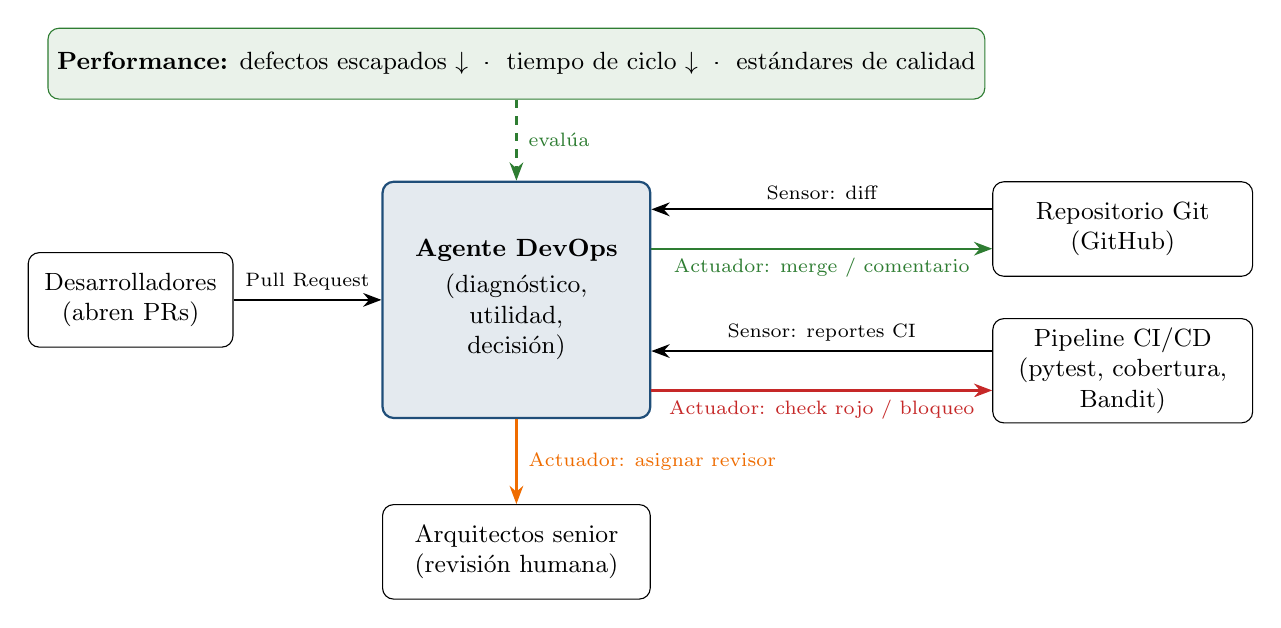
\begin{tikzpicture}[>=Stealth, font=\small,
  caja/.style={draw, rounded corners, align=center, fill=white, minimum height=1.2cm},
  flecha/.style={->, thick}, et/.style={font=\scriptsize, fill=white, inner sep=1pt}]
\node[caja, fill=azul!12, draw=azul, thick, minimum width=3.4cm, minimum height=3cm] (ag) at (0,0)
  {\textbf{Agente DevOps}\\[2pt](diagnóstico,\\utilidad,\\decisión)};
\node[caja, minimum width=2.6cm] (dev) at (-4.9,0) {Desarrolladores\\(abren PRs)};
\node[caja, minimum width=3.3cm] (repo) at (7.7,0.9) {Repositorio Git\\(GitHub)};
\node[caja, minimum width=3.3cm] (ci) at (7.7,-0.9) {Pipeline CI/CD\\(pytest, cobertura,\\Bandit)};
\node[caja, minimum width=3.4cm] (arq) at (0,-3.2) {Arquitectos senior\\(revisión humana)};
\node[caja, fill=verde!10, draw=verde, minimum width=9cm, minimum height=0.9cm] (perf) at (0,3)
  {\textbf{Performance:} defectos escapados $\downarrow$ \;·\; tiempo de ciclo $\downarrow$ \;·\; estándares de calidad};
% desarrolladores
\draw[flecha] (dev.east) -- node[et, above=2pt]{Pull Request} (ag.west);
% repositorio: sensor (arriba) y actuador (abajo)
\draw[flecha] (repo.west |- 0,1.15) -- node[et, above=2pt]{Sensor: diff} (ag.east |- 0,1.15);
\draw[flecha, verde] (ag.east |- 0,0.65) -- node[et, below=2pt, text=verde]{Actuador: merge / comentario} (repo.west |- 0,0.65);
% pipeline: sensor (arriba) y actuador (abajo)
\draw[flecha] (ci.west |- 0,-0.65) -- node[et, above=2pt]{Sensor: reportes CI} (ag.east |- 0,-0.65);
\draw[flecha, rojo] (ag.east |- 0,-1.15) -- node[et, below=2pt, text=rojo]{Actuador: check rojo / bloqueo} (ci.west |- 0,-1.15);
% arquitectos y performance
\draw[flecha, naranja] (ag.south) -- node[et, right=3pt, text=naranja]{Actuador: asignar revisor} (arq.north);
\draw[flecha, dashed, verde] (perf.south) -- node[et, right=3pt, text=verde]{evalúa} (ag.north);
\end{tikzpicture}
\caption{Interacción del Agente DevOps con su entorno.}
\label{fig:contexto}
\end{figure}

% ============================== 3 =========================================
\section{Diseño arquitectónico}

\subsection{Justificación del enfoque}

Se eligió una \textbf{arquitectura basada en utilidad}. Un agente reflejo simple (reglas
\textit{if/else}) no puede equilibrar objetivos en conflicto: tendría que decidir de forma binaria si
un PR de 1200 líneas en el módulo de autenticación ``es aceptable'' o no. Un agente basado en
objetivos solo sabría que la meta es ``PR cerrado'', sin distinguir entre cerrarlo rápido y cerrarlo
bien. La función de utilidad, en cambio, asigna a cada acción un valor numérico que combina
velocidad, riesgo, costo humano y calidad, y permite \emph{auditar} cada decisión.

Además, por ser el entorno parcialmente observable, el agente mantiene un \textbf{modelo del mundo}
que convierte los sensores en una estimación de $\Pdef(s)$. Sobre esta base se añade una \textbf{capa
de restricciones duras} (penalización $w_p$) que impide, sin importar el resto de términos, fusionar
código con pruebas rotas o con vulnerabilidades críticas. La arquitectura queda preparada para
evolucionar a un esquema híbrido: el modelo de riesgo $\Pdef$ es el componente que podría sustituirse
por un modelo de aprendizaje automático entrenado con el historial de incidentes, sin modificar la
capa de utilidad (ver sección~\ref{sec:conclusiones}).

\subsection{Flujo interno de decisión}

\begin{figure}[H]
\centering
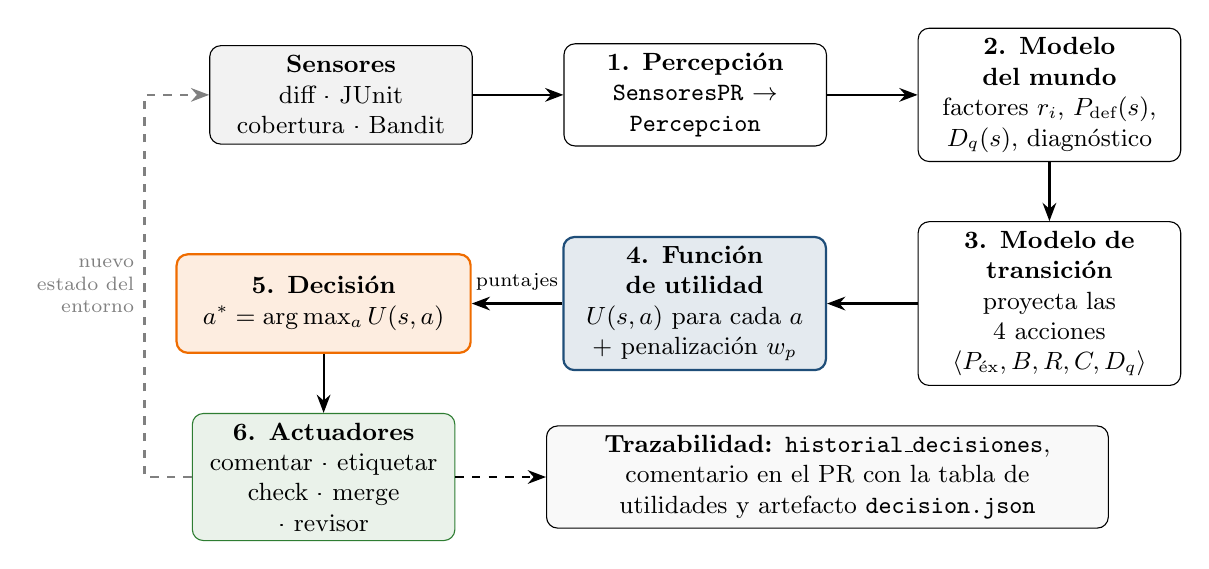
\begin{tikzpicture}[
  node distance=0.75cm and 1.15cm, >=Stealth,
  m/.style={draw, rounded corners, align=center, text width=3.1cm, minimum height=1.25cm, font=\small, fill=white},
  s/.style={m, fill=gray!10},
  u/.style={m, fill=azul!12, draw=azul, thick},
  d/.style={m, fill=naranja!12, draw=naranja, thick},
  a/.style={m, fill=verde!10, draw=verde},
  flecha/.style={->, thick}]
% Sensores
\node[s] (s1) {\textbf{Sensores}\\diff · JUnit\\cobertura · Bandit};
\node[m, right=of s1] (p) {\textbf{1. Percepción}\\\texttt{SensoresPR} $\to$\\\texttt{Percepcion}};
\node[m, right=of p] (mw) {\textbf{2. Modelo del mundo}\\factores $r_i$, $\Pdef(s)$,\\$D_q(s)$, diagnóstico};
\node[m, below=of mw] (tr) {\textbf{3. Modelo de transición}\\proyecta las 4 acciones\\$\langle P_{\text{éx}}, B, R, C, D_q\rangle$};
\node[u, left=of tr] (U) {\textbf{4. Función de utilidad}\\$U(s,a)$ para cada $a$\\+ penalización $w_p$};
\node[d, left=of U, text width=3.5cm] (dec) {\textbf{5. Decisión}\\\mbox{$a^* = \arg\max_a U(s,a)$}};
\node[a, below=of dec] (act) {\textbf{6. Actuadores}\\comentar · etiquetar\\check · merge · revisor};
\node[m, right=of act, text width=6.9cm, fill=gray!5] (log) {\textbf{Trazabilidad:} \texttt{historial\_decisiones}, comentario en el PR con la tabla de utilidades y artefacto \texttt{decision.json}};

\draw[flecha] (s1) -- (p);
\draw[flecha] (p) -- (mw);
\draw[flecha] (mw) -- (tr);
\draw[flecha] (tr) -- (U);
\draw[flecha] (U) -- node[above=1pt, font=\scriptsize]{puntajes} (dec);
\draw[flecha] (dec) -- (act);
\draw[flecha, dashed] (act) -- (log);
\draw[flecha, dashed, gray] (act.west) -- ++(-0.6,0) |- node[pos=0.25, left, font=\scriptsize, align=right]{nuevo\\estado del\\entorno} (s1.west);
\end{tikzpicture}
\caption{Flujo interno del Agente DevOps basado en utilidad.}
\label{fig:arquitectura}
\end{figure}

Los módulos de la figura~\ref{fig:arquitectura} corresponden uno a uno con los métodos de la clase
\texttt{AgenteBasadoEnUtilidad} de la plantilla del taller:

\begin{enumerate}[leftmargin=*]
\item \textbf{Percepción:} \texttt{SensoresPR.a\_percepcion()} normaliza las lecturas del pipeline.
\item \textbf{Modelo del mundo:} \texttt{actualizar\_estado\_interno()} calcula $\Pdef$ y clasifica el PR
      (\texttt{PR\_TRIVIAL}, \texttt{PR\_ESTANDAR}, \texttt{PR\_RIESGOSO}, \texttt{PR\_FALLIDO},
      \texttt{PR\_BLOQUEANTE}).
\item \textbf{Modelo de transición:} \texttt{generar\_estados\_proyectados()} estima el resultado de las
      cuatro acciones. Siempre se generan las cuatro, sin importar el diagnóstico.
\item \textbf{Utilidad:} \texttt{calcular\_utilidad()} aplica la ecuación~\eqref{eq:U}.
\item \textbf{Decisión:} \texttt{seleccionar\_mejor\_accion()} toma el \textit{argmax}.
\item \textbf{Actuadores:} \texttt{ejecutar\_actuador()} y el workflow de GitHub Actions aplican la acción.
\end{enumerate}

% ============================== 4 =========================================
\section{Función de utilidad}

\subsection{Definición formal}

Sea $s$ el estado percibido de un PR y $a \in \mathcal{A} = \{\textsc{merge}, \textsc{corregir},
\textsc{arquitecto}, \textsc{bloquear}\}$. La utilidad de ejecutar $a$ en $s$ es:

\begin{equation}
\label{eq:U}
U(s,a) = w_e\,P_{\text{éx}}(s,a) + w_b\,B(a) - w_r\,R(s,a) - w_c\,C(a) - w_q\,D_q(s,a) - w_p\,\mathbf{1}\big[\text{viola}(s,a)\big]
\end{equation}

\noindent y el agente elige $a^* = \arg\max_{a \in \mathcal{A}} U(s,a)$. Los términos son:

\begin{itemize}[leftmargin=*]
\item $P_{\text{éx}}(s,a) \in [0,1]$: probabilidad de que la acción deje el PR correctamente resuelto.
\item $B(a) \in [0,100]$: beneficio en velocidad de entrega (100 = merge inmediato, 0 = pipeline detenido).
\item $R(s,a) \in [0,1]$: riesgo esperado en producción.
\item $C(a) \in [0,1]$: costo de intervención (tiempo humano de revisión o bloqueo del pipeline).
\item $D_q(s,a) \in [0,1]$: déficit de calidad si el código se fusiona sin cambios (solo aplica a \textsc{merge}).
\item $\mathbf{1}[\text{viola}]$: vale 1 si la acción incumple una política dura de CI/CD.
\end{itemize}

\subsection{Modelo de riesgo $\Pdef(s)$}

Como el entorno es parcialmente observable, la probabilidad de que el PR contenga un defecto se
estima a partir de cinco factores normalizados $r_i(s) \in [0,1]$:

\begin{align}
r_{\text{tests}} &= 1 - \frac{\text{pruebas que pasan}}{\text{pruebas totales}} &
r_{\text{cob}} &= \max\!\Big(0, \frac{0.80 - \text{cob}}{0.80}\Big) \nonumber\\
r_{\text{tam}} &= \min\!\Big(1, \frac{\text{líneas}}{1000}\Big) &
r_{\text{crit}} &= \mathbf{1}[\text{toca módulo crítico}] \nonumber\\
r_{\text{seg}} &= \min\big(1,\; 1.0\,n_{\text{crít}} + 0.5\,n_{\text{alta}} + 0.15\,n_{\text{media}}\big) \nonumber
\end{align}

\begin{equation}
\label{eq:pdef}
\Pdef(s) = \min\Big(1,\; 0.05 + 0.45\,r_{\text{tests}} + 0.15\,r_{\text{cob}} + 0.15\,r_{\text{tam}}
+ 0.10\,r_{\text{crit}} + 0.40\,r_{\text{seg}}\Big)
\end{equation}

\noindent Los módulos críticos se detectan por la ruta del archivo (\texttt{auth}, \texttt{payment},
\texttt{infra}, \texttt{migrations}, \texttt{.github/workflows}, etc.). Si el PR solo modifica
documentación, $r_{\text{tam}} = r_{\text{crit}} = 0$.

El riesgo en producción combina $\Pdef$ con el impacto $I(a)$ de la acción y una exposición
$E(s)$:

\begin{equation}
R(s,a) = \min\big(1,\; \Pdef(s)\cdot I(s,a) + E(s)\big), \qquad
E(s) = \begin{cases} 0.5 & \text{si } n_{\text{crít}} > 0 \text{ y } a \neq \textsc{bloquear}\\ 0 & \text{en otro caso}\end{cases}
\end{equation}

La exposición $E(s)$ modela que un secreto expuesto o una inyección SQL ya constituyen un incidente:
cualquier acción que no detenga el pipeline deja abierta la ventana de explotación.

El déficit de calidad mide el incumplimiento de los estándares del equipo:
\begin{equation}
D_q(s, \textsc{merge}) = \min\Big(1,\; \frac{\max(0,\, 0.70 - \text{cob})}{0.70} + 0.5\,n_{\text{alta}} + 0.1\,n_{\text{media}}\Big)
\end{equation}

\subsection{Proyección de cada acción}

\begin{table}[H]
\centering
\caption{Estados proyectados por el modelo de transición.}
\label{tab:proyeccion}
\small
\begin{tabularx}{\textwidth}{@{}l c c c c X@{}}
\toprule
\textbf{Acción} & $P_{\text{éx}}$ & $B$ & $I$ (impacto) & $C$ & \textbf{Viola política si\ldots} \\
\midrule
\textsc{merge} & $1-\Pdef$ & 100 & 1.0 crítico / 0.6 & 0.0 & pruebas fallan o $n_{\text{crít}}>0$ \\
\textsc{corregir} & 0.90 con hallazgos / 0.50 & 40 & 0.10 & 0.3 & --- \\
\textsc{arquitecto} & 0.97 & 25 & 0.05 & 0.8 & --- \\
\textsc{bloquear} & 0.99 si $n_{\text{crít}}>0$ / 0.30 & 0 & 0 & 0.6 & --- \\
\bottomrule
\end{tabularx}
\end{table}

\textsc{corregir} tiene alta probabilidad de éxito solo cuando existen \emph{hallazgos concretos}
(pruebas que fallan, baja cobertura, alertas): el autor puede arreglarlos con el comentario del bot.
Si el riesgo proviene del tamaño o de la criticidad del módulo, un comentario automático no lo
resuelve y la revisión humana resulta más útil.

\subsection{Pesos y penalizaciones}

\begin{table}[H]
\centering
\caption{Calibración de pesos.}
\label{tab:pesos}
\begin{tabularx}{\textwidth}{@{}c c l X@{}}
\toprule
\textbf{Peso} & \textbf{Valor} & \textbf{Prioridad} & \textbf{Justificación} \\
\midrule
$w_p$ & 1000 & Crítico (restricción) & Nunca fusionar con pruebas rotas o vulnerabilidad crítica. \\
$w_r$ & 400 & Crítico & Un defecto en producción cuesta mucho más que un retraso. \\
$w_q$ & 300 & Alto & Hacer cumplir los estándares de calidad (Performance). \\
$w_e$ & 100 & Alto & Priorizar acciones que realmente resuelven el PR. \\
$w_c$ & 30 & Medio & Penalizar el tiempo de los revisores senior. \\
$w_b$ & 1 & Base & Escala 0--100: recompensa la entrega rápida. \\
\bottomrule
\end{tabularx}
\end{table}

\subsection{Ejemplos de cálculo}

\paragraph{PR-104 (secreto expuesto, 80 líneas).} $r_{\text{seg}}=1$, $r_{\text{tam}}=0.08$, de
modo que $\Pdef = 0.05 + 0.15(0.08) + 0.40(1) = 0.462$.
\begin{align*}
U(\textsc{merge}) &= 100(0.538) + 100 - 400\,(0.462\cdot0.6 + 0.5) - 0 - 0 - 1000 = -1157.08\\
U(\textsc{corregir}) &= 100(0.90) + 40 - 400\,(0.0462 + 0.5) - 30(0.3) = -97.48\\
U(\textsc{arquitecto}) &= 100(0.97) + 25 - 400\,(0.0231 + 0.5) - 30(0.8) = -111.24\\
U(\textsc{bloquear}) &= 100(0.99) + 0 - 0 - 30(0.6) = \mathbf{81.00}
\end{align*}

\paragraph{PR-105 (migración OAuth2, 1200 líneas en \texttt{src/auth}, pruebas en verde).}
$r_{\text{tam}}=1$ y $r_{\text{crit}}=1$, por lo que $\Pdef = 0.05 + 0.15 + 0.10 = 0.30$ e $I=1.0$.
\begin{align*}
U(\textsc{merge}) &= 100(0.70) + 100 - 400(0.30) = 50.00\\
U(\textsc{corregir}) &= 100(0.50) + 40 - 400(0.03) - 30(0.3) = 69.00\\
U(\textsc{arquitecto}) &= 100(0.97) + 25 - 400(0.015) - 30(0.8) = \mathbf{92.00}\\
U(\textsc{bloquear}) &= 100(0.30) - 30(0.6) = 12.00
\end{align*}
Aunque las pruebas pasan, el tamaño y la criticidad hacen que la revisión senior sea la opción
óptima. Esta es exactamente la situación ambigua que una regla \textit{if/else} no resuelve bien.

% ============================== 5 =========================================
\section{Implementación en Python}

\subsection{Estructura del repositorio}

\begin{lstlisting}[language={}, numbers=none]
agente_devops/
  base.py        Plantilla del taller (clase AgenteBasadoEnUtilidad)
  sensores.py    SensoresPR + parsers de git diff, JUnit, coverage y Bandit
  agente.py      AgenteDevOps: modelo del mundo, transicion y actuadores
  kpis.py        Metricas de desempeno
  config.py      Pesos y umbrales calibrados
scripts/
  recolectar_sensores.py   Construye la percepcion en GitHub Actions
  revisar_pr.py            Ejecuta el agente y genera el comentario del PR
simulacion.py    Bateria de 7 casos de prueba + analisis de sensibilidad
tests/           26 pruebas unitarias (pytest), cobertura 97 %
.github/workflows/  ci.yml y agente-pr.yml
\end{lstlisting}

El código conserva la interfaz abstracta de la plantilla y la extiende en dos puntos: la función de
utilidad incorpora los términos $D_q$ y $w_p$, y \texttt{EstadoProyectado} valida que cada variable
esté en su rango. Los parámetros viven en \texttt{config.py}, separados de la lógica, para poder
recalibrar sin tocar el código.

\begin{lstlisting}[caption={Función de utilidad (\texttt{base.py}).}]
def calcular_utilidad(self, estado: EstadoProyectado) -> float:
    p = self.pesos
    utilidad = (
        p["exito"] * estado.probabilidad_exito
        + p["beneficio"] * estado.beneficio_operativo
        - p["riesgo"] * estado.riesgo_impacto
        - p["costo"] * estado.costo_intervencion
        - p["calidad"] * estado.deficit_calidad
        - (p["politica"] if estado.viola_politica else 0.0)
    )
    return round(utilidad, 2)
\end{lstlisting}

\begin{lstlisting}[caption={Modelo de riesgo $\Pdef(s)$ (\texttt{agente.py}).}]
def probabilidad_defecto(self, d):
    r = self.factores_riesgo(d)
    p = config.RIESGO_BASE + sum(config.COEF_RIESGO[k] * v for k, v in r.items())
    return round(_acotar(p), 4)
\end{lstlisting}

\paragraph{Manejo de errores.} Los sensores validan sus rangos (líneas negativas, cobertura fuera de
$[0,1]$, más pruebas fallidas que totales) y lanzan \texttt{ValueError}; el agente rechaza pesos
incompletos; el script de revisión devuelve el código 2 si el JSON de sensores es inválido. Cada
decisión se registra con \texttt{logging} y en \texttt{historial\_decisiones}.

\subsection{Integración con GitHub Actions}

El workflow \texttt{agente-pr.yml} se ejecuta en cada PR y materializa el ciclo PEAS completo:

\begin{enumerate}[leftmargin=*]
\item \textbf{Sensores:} \texttt{git diff --numstat}, \texttt{pytest --junitxml --cov}, \texttt{bandit -f json}.
\item \textbf{Percepción:} \texttt{recolectar\_sensores.py} consolida todo en \texttt{sensores.json}.
\item \textbf{Decisión:} \texttt{revisar\_pr.py} ejecuta el agente y escribe \texttt{decision.json} y \texttt{comentario.md}.
\item \textbf{Actuadores:} publica el comentario con la tabla de utilidades, aplica una etiqueta,
      asigna al arquitecto (variable \texttt{ARQUITECTO\_SENIOR}), fusiona si
      \texttt{AGENTE\_AUTOMERGE=true} y deja el \textit{check} en rojo cuando la decisión es
      \textsc{bloquear} o \textsc{corregir}. Con \textit{branch protection} activa, esto impide el merge.
\end{enumerate}

\noindent Como medida de seguridad, el título del PR (entrada controlada por el usuario) se pasa al
script mediante una variable de entorno y nunca se interpola directamente en el comando, lo que evita
la inyección de comandos en el runner.

% ============================== 6 =========================================
\section{Casos de prueba y métricas}

\subsection{Escenarios}

Se diseñaron siete escenarios. Para cada uno se definió la decisión que tomaría un revisor experto
(oráculo) y si el PR contiene realmente un defecto, con el fin de medir los KPIs.

\begin{table}[H]
\centering
\caption{Matriz de casos de prueba (lecturas de sensores).}
\label{tab:casos}
\small
\begin{tabularx}{\textwidth}{@{}l l >{\raggedright\arraybackslash}X r c r c@{}}
\toprule
\textbf{PR} & \textbf{Tipo} & \textbf{Descripción} & \textbf{Líneas} & \textbf{Pruebas} & \textbf{Cob.} & \textbf{SAST} \\
\midrule
101 & Rutinario & Corrige un typo en \texttt{README.md} & 3 & 42/42 & 85\,\% & --- \\
102 & Rutinario & Exportar reportes a CSV, con pruebas & 150 & 58/58 & 85\,\% & --- \\
103 & Crítico & Nuevo cálculo de descuentos & 200 & 48/60 & 80\,\% & --- \\
104 & Crítico & Conexión a BD con contraseña en el código y SQL concatenado & 80 & 40/40 & 82\,\% & 2 crít. \\
105 & Ambiguo & Migración de sesiones a OAuth2 en \texttt{src/auth} & 1200 & 130/130 & 82\,\% & --- \\
106 & Ambiguo & Plantillas de correo sin pruebas suficientes & 300 & 35/35 & 55\,\% & --- \\
107 & Ambiguo & Carga de archivos con \texttt{subprocess(shell=True)} & 60 & 50/50 & 78\,\% & 1 alta \\
\bottomrule
\end{tabularx}
\end{table}

\subsection{Resultados}

\begin{table}[H]
\centering
\caption{Utilidad calculada para cada acción y decisión del agente.}
\label{tab:resultados}
\footnotesize\setlength{\tabcolsep}{4pt}
\begin{tabular}{@{}l l c r r r r l c@{}}
\toprule
\textbf{PR} & \textbf{Diagnóstico} & $\Pdef$ & \textbf{Merge} & \textbf{Corregir} & \textbf{Arquit.} & \textbf{Bloquear} & \textbf{Decisión} & \textbf{Oráculo} \\
\midrule
101 & TRIVIAL    & 0.050 & \textbf{183.00} & 79.00 & 97.00 & 12.00 & Merge & \checkmark \\
102 & ESTANDAR   & 0.072 & \textbf{175.35} & 78.12 & 96.56 & 12.00 & Merge & \checkmark \\
103 & FALLIDO    & 0.170 & $-857.80$ & \textbf{114.20} & 94.60 & 12.00 & Corregir & \checkmark \\
104 & BLOQUEANTE & 0.462 & $-1157.08$ & $-97.48$ & $-111.24$ & \textbf{81.00} & Bloquear & \checkmark \\
105 & RIESGOSO   & 0.300 & 50.00 & 69.00 & \textbf{92.00} & 12.00 & Arquitecto & \checkmark \\
106 & RIESGOSO   & 0.142 & 87.48 & \textbf{115.32} & 95.16 & 12.00 & Corregir & \checkmark \\
107 & RIESGOSO   & 0.263 & $-39.31$ & \textbf{110.48} & 92.76 & 12.00 & Corregir & \checkmark \\
\bottomrule
\end{tabular}
\end{table}

\begin{itemize}[leftmargin=*]
\item \textbf{Rutinarios (101, 102):} el riesgo es bajo y el merge obtiene casi el doble de utilidad
      que cualquier alternativa; el agente libera a los revisores de este trabajo.
\item \textbf{Críticos (103, 104):} la penalización $w_p$ hace imposible el merge. En el PR-103 el
      fallo es concreto y corregible, así que se solicitan correcciones; en el PR-104 la exposición
      $E(s)$ hace que solo bloquear tenga utilidad positiva.
\item \textbf{Ambiguos (105--107):} el PR-105 pasa todas las pruebas, pero su tamaño y criticidad lo
      envían a un arquitecto. En los PR-106 y 107 el término $D_q$ reduce la utilidad del merge por
      debajo de \textsc{corregir}, porque hay hallazgos concretos que el autor puede resolver.
\end{itemize}

\subsection{Indicadores clave de desempeño (KPIs)}

\begin{table}[H]
\centering
\caption{KPIs obtenidos en la simulación.}
\label{tab:kpis}
\begin{tabularx}{\textwidth}{@{}l r X@{}}
\toprule
\textbf{KPI} & \textbf{Valor} & \textbf{Relación con Performance} \\
\midrule
Precisión frente al oráculo experto & 100\,\% & Calidad de las decisiones \\
Defectos escapados a producción & 0 de 4 & Reducción de fallos tras el despliegue \\
\textit{Recall} de defectos & 100\,\% & Todo PR defectuoso fue detenido \\
Tasa de merge automático & 28.6\,\% & Trabajo humano ahorrado \\
Tasa de escalamiento a senior & 14.3\,\% & Solo el caso de alto impacto \\
Tiempo de ciclo promedio & 211.4 min & Frente a 720 min si un senior revisa todo: $-70.6\,\%$ \\
\bottomrule
\end{tabularx}
\end{table}

\noindent El tiempo de ciclo se simuló con valores de referencia por acción: merge 5 min, bloqueo
30 min, corrección del autor 240 min y revisión senior 720 min.

\subsection{Análisis de sensibilidad del peso de riesgo}

Para validar la calibración se repitió la simulación variando $w_r$:

\begin{table}[H]
\centering
\caption{Sensibilidad de las decisiones frente a $w_r$.}
\label{tab:sensibilidad}
\small\setlength{\tabcolsep}{4pt}
\begin{tabular}{@{}r c c c r p{5.2cm}@{}}
\toprule
$w_r$ & \textbf{Precisión} & \textbf{Merge auto} & \textbf{Escapados} & \textbf{Ciclo (min)} & \textbf{Errores} \\
\midrule
50  & 71.4\,\% & 42.9\,\% & 0 & 139.3 & PR-104 no se bloquea; PR-105 se fusiona \\
100 & 85.7\,\% & 42.9\,\% & 0 & 109.3 & PR-105 se fusiona sin revisión senior \\
200 & 85.7\,\% & 42.9\,\% & 0 & 109.3 & PR-105 se fusiona sin revisión senior \\
\textbf{400} & \textbf{100\,\%} & 28.6\,\% & 0 & 211.4 & --- \\
800 & 100\,\% & 28.6\,\% & 0 & 211.4 & --- \\
\bottomrule
\end{tabular}
\end{table}

Con un peso de riesgo bajo, el agente prioriza la velocidad: fusiona sin revisión una migración de
1200 líneas en el módulo de autenticación y, con $w_r=50$, ni siquiera bloquea un secreto expuesto.
A partir de $w_r=400$ las decisiones son estables, por lo que ese valor es el punto en que el agente
resuelve correctamente el dilema sin sacrificar más velocidad de la necesaria. La política dura $w_p$
garantiza que, incluso con pesos mal calibrados, no se fusione código con pruebas rotas.

\subsection{Pruebas unitarias}

La suite de \texttt{pytest} (26 pruebas, 97\,\% de cobertura) verifica los siete escenarios, las
propiedades de seguridad (``nunca fusionar con una vulnerabilidad crítica'' para distintos tamaños de
PR), la monotonía del riesgo frente al tamaño, la fórmula de utilidad, la validación de entradas y
los \textit{parsers} de los artefactos del pipeline. El workflow \texttt{ci.yml} ejecuta la suite, Bandit
y la simulación en cada \textit{push}.

% ============================== 7 =========================================
\section{Conclusiones y trabajo futuro}
\label{sec:conclusiones}

\begin{itemize}[leftmargin=*]
\item El modelo PEAS permitió delimitar desde el inicio qué percibe el agente (artefactos del
      pipeline) y cómo actúa (API de GitHub), lo que se tradujo directamente en el código.
\item La función de utilidad resuelve el dilema velocidad--riesgo de forma cuantitativa y auditable:
      cada comentario en el PR muestra los puntajes de las cuatro acciones.
\item Las restricciones duras ($w_p$) y la exposición $E(s)$ evitan que el equilibrio de pesos
      permita acciones inaceptables, como fusionar un secreto expuesto.
\item El agente resolvió sin intervención humana 6 de los 7 PRs simulados (85.7\,\%: merge,
      corrección o bloqueo) y solo escaló el caso de alto impacto, reduciendo el tiempo de ciclo un 70.6\,\%.
\end{itemize}

\paragraph{Trabajo futuro.}
(1) Evolucionar hacia una arquitectura híbrida, reemplazando los coeficientes $\alpha_i$ de
$\Pdef$ por un modelo de aprendizaje automático entrenado con el historial de incidentes del
repositorio, y usar como elemento de crítica la tasa de reversiones (\textit{reverts}) tras el
despliegue.
(2) Calcular la cobertura solo sobre las líneas modificadas (\textit{diff coverage}).
(3) Incorporar un sistema multiagente (analista de seguridad, crítico de rendimiento y gerente de
merge) orquestado con LangGraph, como propone el ejercicio 3 del taller.

\begin{thebibliography}{9}
\bibitem{russell} S. Russell y P. Norvig, \textit{Artificial Intelligence: A Modern Approach}, 4.ª ed. Pearson, 2021.
\bibitem{taller} \textit{Taller de Ingeniería de Agentes Inteligentes: de los fundamentos a los sistemas multiagente}. Material de clase, noviembre de 2026.
\bibitem{gha} GitHub, ``GitHub Actions documentation''. \url{https://docs.github.com/actions}
\bibitem{bandit} PyCQA, ``Bandit: security linter for Python''. \url{https://bandit.readthedocs.io}
\end{thebibliography}

\end{document}
